\section{Sistema de hormigas Elitista}



\subsection{Introducción}

Uno de los problemas más estudiados por los etólogos ha sido entender cómo animales con capacidades visuales
limitadas, como las hormigas, logran establecer rutas eficientes desde su colonia para conseguir recursos y volver.
Se ha descubierto que la forma más usual para comunicar información entre los individuos sobre los caminos, 
y que se usa para decidir a dónde ir, se basa en el rastro de feromonas.
El movimiento de hormigas deposita esta sustancia en el suelo, marcando el sendero.
Este mecanismo genera un proceso de retroalimentación positiva: de tal forma que cuanto más sigan las hormigas 
un rastro, más atractivo se vuelve ese rastro para ser seguido. 
En concreto, este comportamiento colectivo se caracteriza porque la probabilidad de que una hormiga escoja 
un camino aumenta en función del número de individuos que ya han transitado esa misma ruta.

\subsection{Sistema de Hormigas}

En primer lugar vamos a utilizar el problema del viajante de comercio (TSP) como caso de estudio para
implementar nuestro sistema de hormigas elitista. 
El TSP es un problema clásico de optimización combinatoria que busca encontrar la ruta más corta 
que visite un conjunto de ciudades exactamente una vez y regrese a la ciudad de origen.

Dado un conjunto de n ciudades, denominamos $d_{ij}$ a la longitud del camino entre la ciudades i y j,
que suele ser la distancia euclídea. Este conjunto de ciudades y caminos viene representado por un grafo (N, E),
donde N es el conjunto de nodos (ciudades) y E el conjunto de aristas (caminos entre ciudades).

Denominamos $b_i(t)$ el número total de hormigas en la ciudad i en el tiempo t y $m = \sum_{i=1}^{n} b_i(t)$ 
el número total de hormigas en el tiempo t.
Cada hormiga dispone de las siguientes características:
\begin{itemize}
    \item Escoge la ciudad siguiente con una probabilidad, que es función de la cantidad de feromona en el camino y de la distancia a la ciudad siguiente.
    \item Obligamos a que realice recorridos válidos, prohibiendo las transiciones a pueblos ya visitados hasta que se complete un recorrido, mediante una lista tabú.
    \item Cuando se completa un recorrido, deposita una sustancia llamada rastro en cada arista visitada.
\end{itemize}

Sea $\tau_{ij}(t)$ la cantidad de feromona en el camino entre las ciudades i y j en el tiempo t.
Cada hormiga en el tiempo t, debe escoger la siguiente ciudad, donde estará en tiempo t+1.
Por lo tanto, si llamamos a una iteración del algoritmo a los m movimientos realizados por las m hormigas en el intervalo (t, t+1), 
entonces cada n iteraciones del algoritmo, cada hormiga ha completado un recorrido, lo que denominaremos ciclo.

En cada ciclo la intensidad del camino se actualiza de la siguiente forma:
\begin{equation}
    \tau_{ij}(t+n) = \rho \cdot \tau_{ij}(t) + \Delta \tau_{ij}
\end{equation}
donde $0 < \rho < 1$ es un coeficiente tal que $1 - \rho$ representa la evaporación del camino entre t y t+n, y
\begin{equation}
   \Delta \tau_{ij} = \sum_{k=1}^{m} \Delta \tau_{ij}^k
\end{equation}
donde $\Delta \tau_{ij}^k$ es la cantidad por unidad de longitud de feromona que la hormiga k deposita en el camino entre las ciudades i y j, 
entre el tiempo t y t+n.
Esta cantidad se define como:
\begin{equation}
    \Delta \tau_{ij}^k = \begin{cases}
    Q / L_k & \text{si la hormiga } k \text{ utiliza el camino } (i, j) \text{ en su recorrido}\\
    0 & \text{en otro caso}
    \end{cases}
\end{equation}
donde Q es una constante y $L_k$ la longitud del recorrido realizado por la hormiga k.

Con el objetivo de satisfacer la restricción de que cada hormiga debe visitar todas las n diferentes ciudades, asociamos a cada hormiga
una lista tabú que almacena las ciudades ya visitadas por esa hormiga.
Cuando se completa un ciclo, la lista tabú se utiliza para calcular la solución actual de cada hormiga.
Luego, la lista se vacía y cada hormiga comienza un nuevo ciclo.

Llamamos visibilidad, $n_{ij}$, a la distancia inversa entre las ciudades i y j, $\frac{1}{d_{i,j}}$. 
Esta cantidad no se modifica durante la ejecución del algoritmo y representa la información heurística disponible para las hormigas.

Definimos la probabilidad de transición de una ciudad i a una ciudad j para la hormiga k en el tiempo t como:
\begin{equation}
    p_{ij}^k = \begin{cases}
    \frac{[\tau_{ij}(t)]^{\alpha} \cdot [n_{ij}]^{\beta}}{\sum_{l \in \text{allowed}_k} [\tau_{il}(t)]^{\alpha} \cdot [n_{il}]^{\beta}} & \text{si } j \in \text{allowed}_k\\
    0 & \text{en otro caso}
    \end{cases}
    \label{eq}
\end{equation}
donde $\text{allowed}_k$ es el conjunto de ciudades que la hormiga k no ha visitado aún, y $\alpha$ y $\beta$ son parámetros que controlan la
importancia relativa entre la feromona y la visibilidad.
Por lo tanto, esta probabilidad es un equilibrio entre la visibilidad, que indica que se deben elegir las ciudades más cercanas con mayor probabilidad,
y la intensidad del rastro en el tiempo t, que indica que si en la arista (i, j) ha habido mucho tráfico, entonces ese camino es más atractivo.

\subsection{Algoritmo}

El algoritmo comienza con una fase de inicialización, donde las hormigas se posicionan en diferentes ciudades y se establece la intensidad inicial de feromona en cada arista del grafo
mediante $\tau_{ij}(0)$. Inicializamos el primer elemento de la lista tabú de cada hormiga con la ciudad donde se encuentra.

Luego, cada hormiga se moverá desde la ciudad i a la ciudad j según la probabilidad de transción y tras n iteraciones todas las hormigas habrán completado un ciclo y sus listas tabú contendrán un recorrido completo.
En este punto, para cada hormiga k se actualiza $L_k$ y la intensidad de feromona en cada arista del grafo según la fórmula dada anteriormente.
Además, se guarda el camino más corto encontrado, $min_k L_k, \quad k = 1,...,m$.
Este proceso se repite hasta que se cumple un criterio de parada, como alcanzar un número máximo de ciclos, $NC_{MAX}$ o todas las hormigas convergen a la misma solución.

Formalmente, el algoritmo se puede describir con los siguientes pasos:
\begin{enumerate}
    \item Inicialización: \\
    \hspace*{0.25cm} Definimos t := 0. \\
    \hspace*{0.25cm} Definimos NC := 0. \\
    \hspace*{0.25cm} Para cada arco (i, j) definimos la intensidad $\tau_{ij}(0) = c$ y $\Delta \tau_{ij} = 0$. \\
    \hspace*{0.25cm} Colocar las m hormigas en los n nodos.
    \item Sea s := 1. \\
    Para k = 1 hasta m hacer \\
    \hspace*{0.25cm} Colocar la ciudad inicial de la hormiga k en la lista tabú, $tabu_k(s)$. 

    \item Repetir hasta que la lista tabú se complete: \\
    Definimos s := s+1 \\
    Para k = 1 hasta m hacer \\
    \hspace*{0.25cm} Elegir la ciudad j a la que moverse con probabilidad $p_{ij}^k(t)$. \\
    \hspace*{0.25cm} Mover la hormiga k a la ciudad j. \\
    \hspace*{0.25cm} Colocar la ciudad j en la lista tabú, $tabu_k(s)$. 
    
    \item Para k = 1 hasta m hacer \\
    \hspace*{0.25cm} Mover la hormiga k de $tabu_k(n)$ a $tabu_k(1)$. \\
    \hspace*{0.25cm} Calcular la longitud del recorrido descrito por la hormiga k, $L_k$. \\
    \hspace*{0.25cm} Actualizar el camino más corto encontrado. \\
    \hspace*{0.25cm} Para cada arco (i, j) del grafo hacer \\
    \hspace*{0.25cm} Para k = 1 hasta m hacer 
    \begin{equation*}
        \Delta \tau_{ij}^k = \begin{cases}
        Q / L_k & \text{si } (i, j) \in \text{ciclo descrito por } tabu_k \\
        0 & \text{en otro caso}
        \end{cases}
    \end{equation*}

    \hspace*{0.25cm} $\Delta \tau_{ij} := \Delta \tau_{ij} + \Delta \tau_{ij}^{k}$

    \item Para cada arco (i, j) calcular $\tau_{ij}(t+n) = \rho \cdot \tau_{ij}(t) + \Delta \tau_{ij}$. \\
    Definir t := t + n. \\
    Definir NC := NC + 1. \\
    Para cada arco (i, j) definir $\Delta \tau_{ij} := 0$. 

    \item Si $(NC < NC_{MAX})$ y no todas las hormigas han convergido a la misma solución \\
    entonces \\
    \hspace*{0.25cm} Vaciar todas las listas tabú. \\
    \hspace*{0.25cm} Ir al paso 2. \\
    sino \\
    \hspace*{0.25cm} Imprimir el ciclo más corto encontrado. \\
    \hspace*{0.25cm} Parar.

\end{enumerate}

\subsubsection{Estrategia elitista}

Para mejorar el rendimiento del algoritmo, implementamos una estrategia elitista. 
Para ello añadimos al camino de cada arco del mejor ciclo la cantidad $e \cdot Q/L^{*}$, donde e es el número de hormigas elitistas y $L^{*}$ la longitud del mejor ciclo encontrado hasta el momento.
De esta forma, se refuerza el camino del mejor ciclo, acelerando la convergencia del algoritmo.
\subsection{Implementación}

Para validar el funcionamiento del Sistema de Hormigas Elitista, se ha realizado una implementación práctica en lenguaje Python. El desarrollo parte de los requisitos establecidos en el enunciado de la Práctica 9, evolucionando desde la resolución del problema base hacia una propuesta experimental multi-objetivo.

\subsubsection{Descripción del Problema y Entorno}

El problema a resolver es el \textbf{Problema de Asignación Generalizado} descrito en el enunciado de la práctica. Este escenario plantea la necesidad de asignar un conjunto de $N=4$ tareas, denotadas como $T_i$ ($i=\{1,..,4\}$), a un conjunto de $M=5$ operarios, denotados como $O_j$ ($j=\{1,..,5\}$).

El modelo está sujeto a las siguientes restricciones y parámetros definidos en la documentación:
\begin{itemize}
    \item \textbf{Restricción de Unicidad:} Cada tarea debe ser realizada por un único operario.
    \item \textbf{Restricción de Capacidad:} Aunque un operario puede realizar múltiples tareas, la suma de los tiempos requeridos por estas ($r_i$) no puede exceder el tiempo total disponible de dicho operario ($d_j$).
    \item \textbf{Función de Coste:} Existe un coste $c_{ij}$ asociado a que el operario $j$ realice la tarea $i$.
\end{itemize}

El objetivo fundamental estipulado es encontrar la asignación válida que minimice el coste total. No obstante, en esta implementación hemos decidido ir un paso más allá de lo solicitado: además de resolver el problema mono-objetivo original, hemos introducido artificialmente un segundo objetivo de optimización (equilibrio de carga) para testar la flexibilidad del algoritmo en entornos multi-objetivo.

Los datos utilizados se corresponden fielmente con la tabla proporcionada en el enunciado, modelados computacionalmente mediante \texttt{NumPy}:

\begin{equation}
C_{ij} (\text{Costes}) = \begin{pmatrix}
2 & 3 & 4 & 1 \\
3 & 2 & 3 & 2 \\
2 & 2 & 1 & 2 \\
3 & 3 & 3 & 3 \\
2 & 1 & 2 & 2
\end{pmatrix}
\end{equation}

\begin{equation}
r_{i} (\text{T. Requerido}) = [3, 2, 2, 3], \quad
d_{j} (\text{T. Disponible}) = [4, 5, 3, 4, 4]
\end{equation}

\subsubsection{Enfoque mono-objetivo: (Elitist Ant System)}

En esta primera fase, nos ceñimos estrictamente al objetivo del enunciado: minimizar el coste total ($f_1 = \sum c_{ij}$). Se implementó el algoritmo descrito en el apartado 3.3, definiendo la información heurística $\eta_{ij}$ como la inversa del coste ($1/c_{ij}$), tal que las hormigas tiendan a escoger las asignaciones más económicas. Se aplicó la estrategia elitista para reforzar el mejor camino global encontrado en cada iteración.

\subsubsection{Extensión multi-objetivo (MOACO y MAS)}

Para extender la práctica y analizar el comportamiento de las metaheurísticas ante conflictos de objetivos, definimos un segundo objetivo no presente en el enunciado original:
\begin{itemize}
    \item \textbf{Objetivo 1 ($f_1$):} Minimizar Coste Total (Objetivo original).
    \item \textbf{Objetivo 2 ($f_2$):} Minimizar el Desequilibrio de Carga (Desviación típica del tiempo de trabajo entre operarios).
\end{itemize}

Se implementaron dos variantes para resolver este problema bi-objetivo:
\begin{enumerate}
    \item \textbf{Simple MOACO:} Utiliza un archivo externo para almacenar el Frente de Pareto.
    \item \textbf{MAS (Multi-Objective Ant System):} Asigna pesos variables $\lambda$ a cada hormiga para equilibrar la importancia de ambos objetivos.
\end{enumerate}
\subsubsection{Resultados Experimentales}

El primer análisis se realizó utilizando estrictamente las matrices de costes y tiempos proporcionadas en el enunciado de la Práctica 9. Tras ejecutar tanto la variante Mono-objetivo como las variantes Multi-objetivo (MOACO y MAS), se observó un fenómeno de convergencia unificada.

\begin{itemize}
    \item \textbf{Solución Obtenida:} Todos los algoritmos convergieron a la misma solución global:
    \begin{itemize}
        \item Coste Total ($f_1$): \textbf{6} (Mínimo teórico).
        \item Desequilibrio ($f_2$): \textbf{1.0954} (Desviación típica).
    \end{itemize}
\end{itemize}

Este comportamiento se debe a la topología específica de los datos de entrada. En esta instancia del problema GAP, los objetivos resultaron ser no conflictivos. La asignación de tareas a los operarios más eficientes en costes minimizando $f_1$ generó, de manera colateral, una distribución de carga que no violaba las restricciones y mantenía un desequilibrio bajo. Al no existir conflicto entre ahorrar dinero y equilibrar carga, el Frente de Pareto teórico colapsó en un único punto dominante, impidiendo visualizar una curva de compromiso trade-off real.


Uno de los aspectos críticos en la validación del algoritmo es asegurar que la solución encontrada no solo minimiza la función objetivo, sino que respeta estrictamente las restricciones de capacidad del problema GAP.A primera vista, una inspección de la matriz de costes $C_{ij}$ sugeriría que el coste mínimo teórico podría ser $f_1 = 5$. Este valor se obtiene aplicando una estrategia \textit{greedy}, seleccionando el mínimo absoluto de cada tarea sin considerar el consumo de recursos. Sin embargo, como se ilustra en la Figura \ref{fig:gap_analysis}, esta combinación es inviable:

\begin{figure}[h]
    \centering
    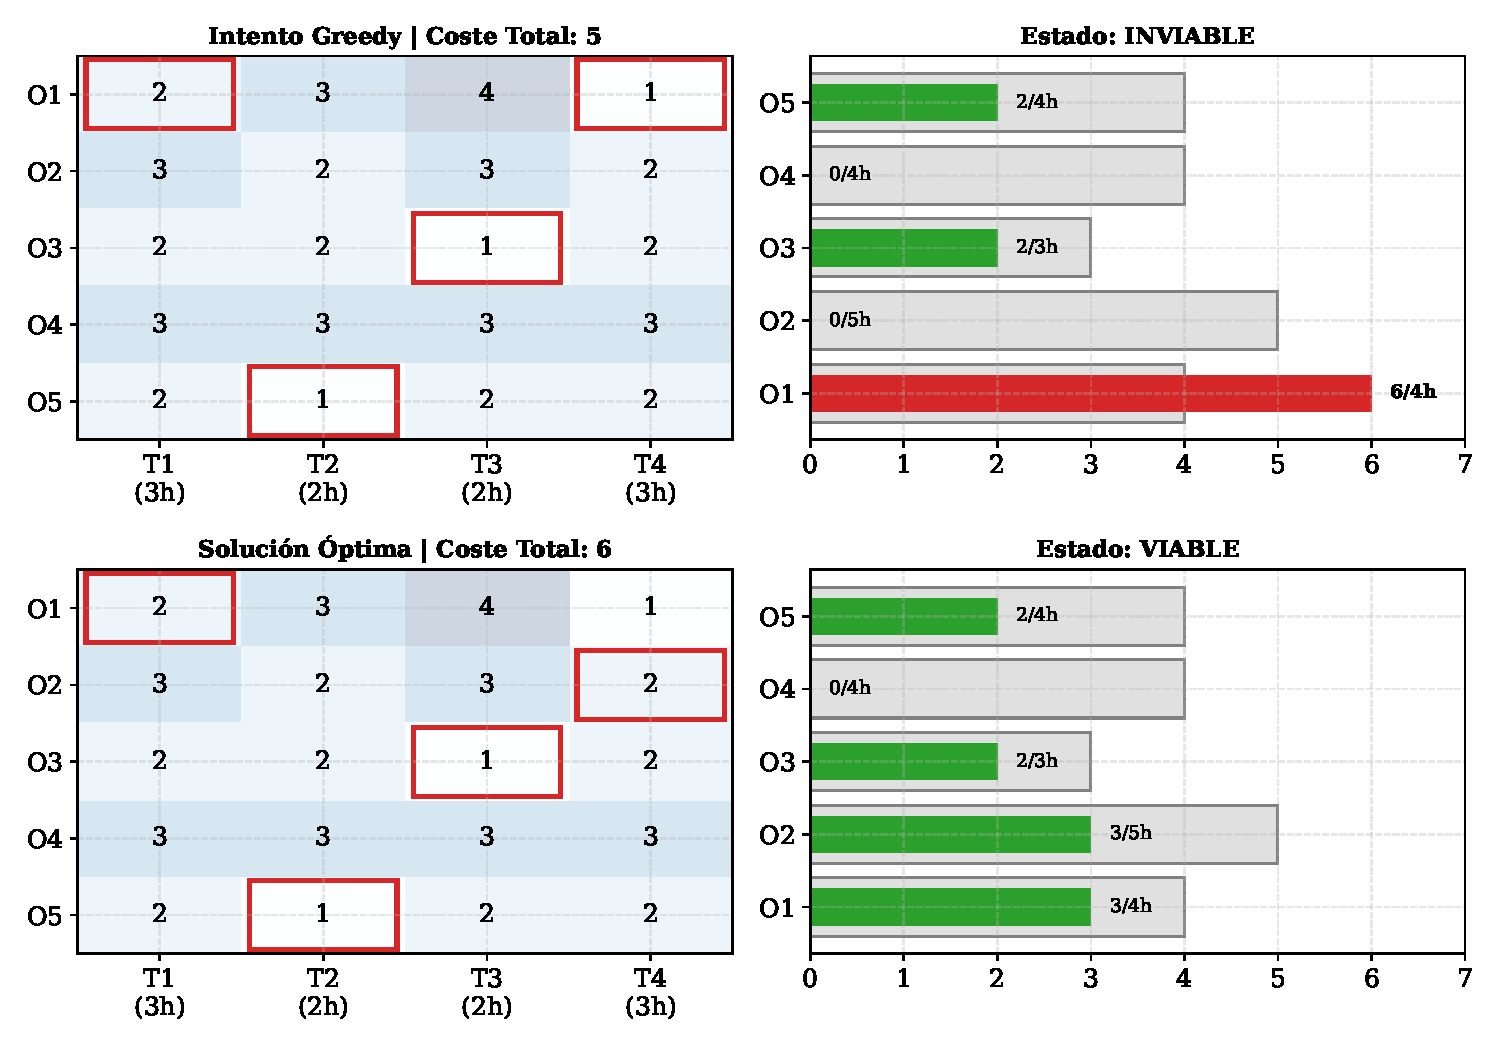
\includegraphics[width=1.0\textwidth]{img/explicacion_sol_ants.pdf}
    \caption{Comparativa entre la selección Greedy y la solución óptima. Sumando los mínimos absolutos viola la capacidad del $O_1$.}
    \label{fig:gap_analysis}
\end{figure}

Por lo tanto, la solución mínima viable de este problema es $f_1 = 6$ tan y como han indicado los tres algoritmos implementados en la práctica. A continuación decidimos crear otro escenario donde las habilidades de los operarios eran menos regulares dando a lugar a un frente de pareto para los algoritmos multiobjetivo.

\textbf{Validación Adicional: Escenario de Conflicto}

Dado que los datos originales no permitían apreciar la capacidad del algoritmo para gestionar objetivos contrapuestos, se diseñó un segundo escenario experimental. El objetivo fue forzar la aparición de un Frente de Pareto real modificando los datos de entrada para generar un conflicto explícito entre Coste y Equilibrio.
Se definió un problema con $N=8$ tareas y $M=3$ operarios con perfiles extremos:
\begin{itemize}
    \item \textbf{Operario 1 (barato):} Coste muy bajo ($c=1$) pero alta probabilidad de saturación.
    \item \textbf{Operario 2 (medio):} Coste moderado ($c=4$).
    \item \textbf{Operario 3 (caro):} Coste alto ($c=8$), su uso es necesario para equilibrar la carga pero penaliza el coste.
\end{itemize}

Al ejecutar el algoritmo MOACO sobre este nuevo conjunto de datos, se obtuvo un conjunto de soluciones no dominadas diverso, tal como se muestra en la Figura \ref{fig:pareto}.

\begin{figure}[H]
    \centering
    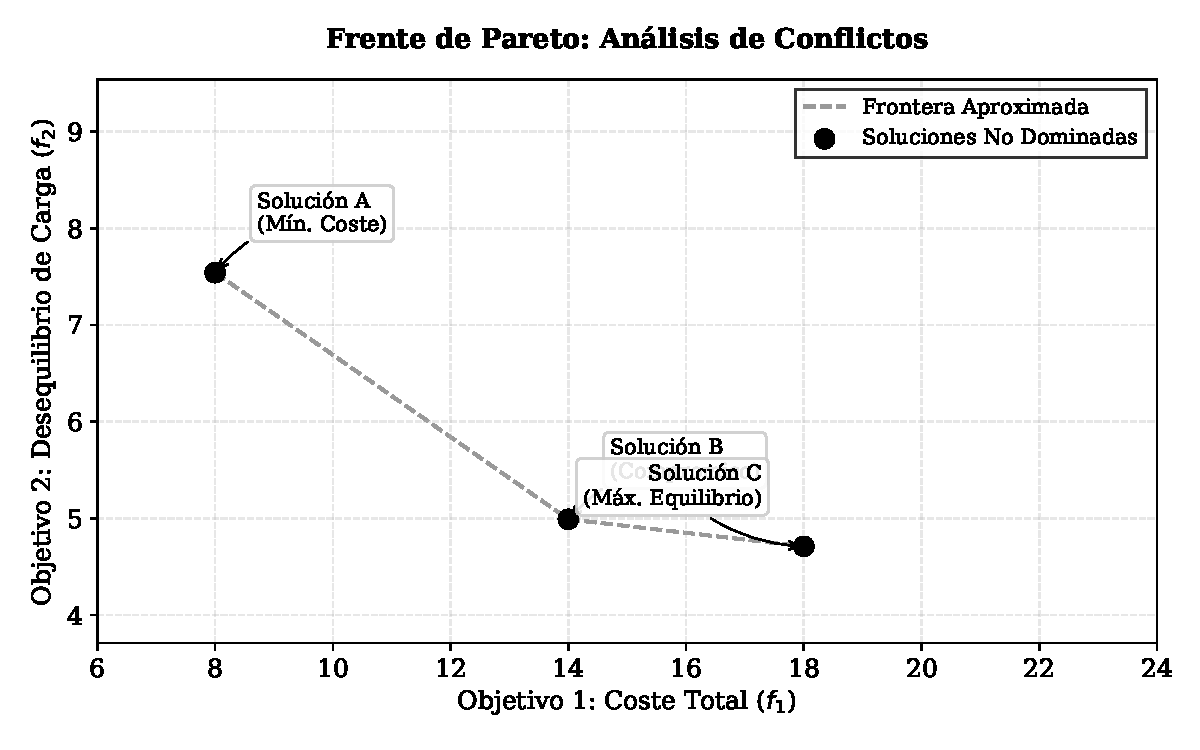
\includegraphics[width=0.7\textwidth]{img/ants_results.pdf}
    \caption{Frente de Pareto obtenido en el escenario de conflicto. Se observa la curva de compromiso entre el Coste Total y el Desequilibrio de Carga.}
    \label{fig:pareto}
\end{figure}

A diferencia del caso anterior, aquí se observan claramente tres regiones de decisión:
\begin{enumerate}
    \item \textbf{Región de mínimo coste ($f_1 \approx 8$):} El algoritmo asigna casi todo al Operario 1. El coste es mínimo, pero el desequilibrio ($f_2$) se dispara por encima de 7.5.
    \item \textbf{Región de compromiso ($f_1 \approx 14$):} Se empieza a derivar trabajo al Operario 2. El coste sube, pero el desequilibrio mejora notablemente.
    \item \textbf{Región de máximo equilibrio ($f_1 \approx 18$):} Se utiliza al Operario 3. Es la opción más cara, pero logra la distribución de trabajo más equitativa posible ($f_2 < 4.8$).
\end{enumerate}

La segunda fase experimental valida la robustez de la implementación, demostrando su capacidad para mantener la diversidad poblacional y hallar soluciones de compromiso en escenarios de conflicto real, superando así las limitaciones observadas en los datos originales. Por otro lado, el análisis de la Figura \ref{fig:gap_analysis} justifica estructuralmente el resultado obtenido: mientras que una estrategia greedy alcanzaría un coste teórico de 5 a expensas de violar la capacidad del Operario 1 (quien recibiría 6 horas de carga frente a sus 4 disponibles), el sistema converge correctamente hacia el óptimo factible de coste 6, priorizando el cumplimiento estricto de las restricciones mediante la reasignación eficiente de recursos.